\documentclass{article}
\usepackage{tikz}
\usetikzlibrary{arrows.meta}

\begin{document}

\begin{figure}[h]
    \centering
    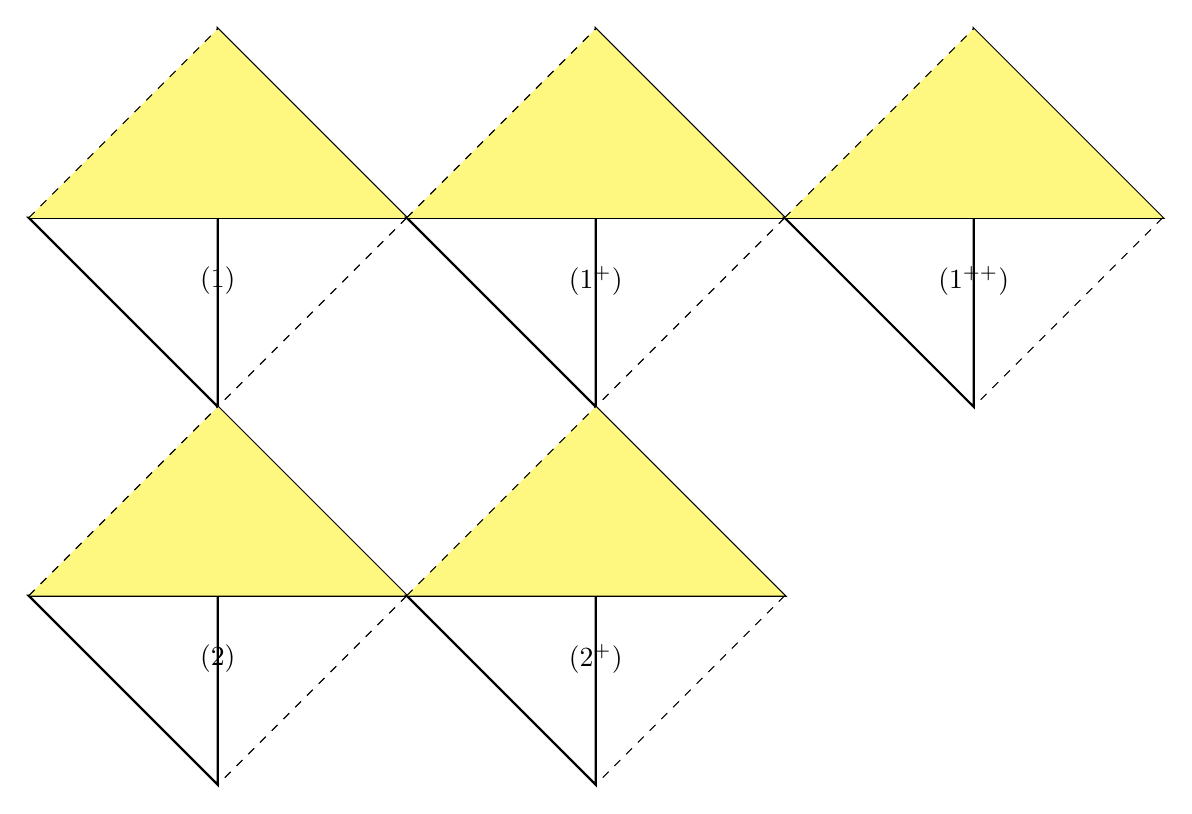
\begin{tikzpicture}[scale=0.8]
        % Define coordinates for the vertices of the regions
        \coordinate (A) at (-3,0);
        \coordinate (B) at (3,0);
        \coordinate (C) at (0,3);
        \coordinate (D) at (0,-3);
        
        % Draw the outer rectangle
        \draw[thick] (A) -- (B) -- (C) -- (D) -- cycle;
        
        % Fill the yellow region
        \fill[yellow!50] (A) -- (B) -- (C) -- cycle;
        
        % Draw the dashed lines
        \draw[dashed] (A) -- (C);
        \draw[dashed] (B) -- (D);
        
        % Label the region
        \node at (0,-1) {$(1)$};
        
        % Repeat for other regions
        \begin{scope}[xshift=6cm]
            \coordinate (A) at (-3,0);
            \coordinate (B) at (3,0);
            \coordinate (C) at (0,3);
            \coordinate (D) at (0,-3);
            
            \draw[thick] (A) -- (B) -- (C) -- (D) -- cycle;
            \fill[yellow!50] (A) -- (B) -- (C) -- cycle;
            \draw[dashed] (A) -- (C);
            \draw[dashed] (B) -- (D);
            \node at (0,-1) {$(1^{+})$};
        \end{scope}
        
        \begin{scope}[xshift=12cm]
            \coordinate (A) at (-3,0);
            \coordinate (B) at (3,0);
            \coordinate (C) at (0,3);
            \coordinate (D) at (0,-3);
            
            \draw[thick] (A) -- (B) -- (C) -- (D) -- cycle;
            \fill[yellow!50] (A) -- (B) -- (C) -- cycle;
            \draw[dashed] (A) -- (C);
            \draw[dashed] (B) -- (D);
            \node at (0,-1) {$(1^{++})$};
        \end{scope}
        
        \begin{scope}[yshift=-6cm]
            \coordinate (A) at (-3,0);
            \coordinate (B) at (3,0);
            \coordinate (C) at (0,3);
            \coordinate (D) at (0,-3);
            
            \draw[thick] (A) -- (B) -- (C) -- (D) -- cycle;
            \fill[yellow!50] (A) -- (B) -- (C) -- cycle;
            \draw[dashed] (A) -- (C);
            \draw[dashed] (B) -- (D);
            \node at (0,-1) {$(2)$};
        \end{scope}
        
        \begin{scope}[xshift=6cm,yshift=-6cm]
            \coordinate (A) at (-3,0);
            \coordinate (B) at (3,0);
            \coordinate (C) at (0,3);
            \coordinate (D) at (0,-3);
            
            \draw[thick] (A) -- (B) -- (C) -- (D) -- cycle;
            \fill[yellow!50] (A) -- (B) -- (C) -- cycle;
            \draw[dashed] (A) -- (C);
            \draw[dashed] (B) -- (D);
            \node at (0,-1) {$(2^{+})$};
        \end{scope}
    \end{tikzpicture}
    
    \caption{Region $M^{\rm I}(i)$ of possible $t$, for $i=\bullet$ in regions labeled by $-1^*$, $1^*$, $2^*$.}
    \label{fig:regions}
\end{figure}

\end{document}